\documentclass{article}

% Language setting
% Replace `english' with e.g. `spanish' to change the document language
\usepackage[portuguese]{babel}

% Set page size and margins
% Replace `letterpaper' with`a4paper' for UK/EU standard size
\usepackage[letterpaper,top=2cm,bottom=2cm,left=3cm,right=3cm,marginparwidth=1.75cm]{geometry}
\newtheorem{exmp}{Exemplo}
% Useful packages
\usepackage{amsmath}
\usepackage{graphicx}
\usepackage[colorlinks=true, allcolors=blue]{hyperref}

\title{Potenciação de números naturais}
\author{Télico Oliveira}

\begin{document}
\maketitle
\section{Exemplo inicial}
Um grupo de adolescentes resolveu doar roupas para uma campanha do agasalho. O organizador doou 2 sacos de roupas e cobertores e convidou 2 pessoas a fazerem a mesma doação. Em seguida, cada uma delas convidou também as outras 2 pessoas. 
Calcule quantas sacolas foram arrecadadas após 4 etapas de arrecadação. 
\subsection{Resolução}
Podemos fazer um diagrama para auxiliar na resolução do problema. 
Cada multiplicação que aparece nessa situação tem fatores iguais. Essas multiplicações com fatores iguais podem ser representadas pela operação de potenciação. 
\begin{figure}[htbp]
    \centering
    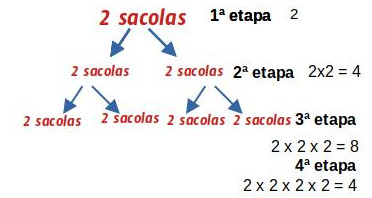
\includegraphics[scale=0.8]{potenciacao1.jpg}
    
    \label{fig:my_label}
\end{figure}
\subsection{Regra}
\begin{figure}[htbp]
    \centering
    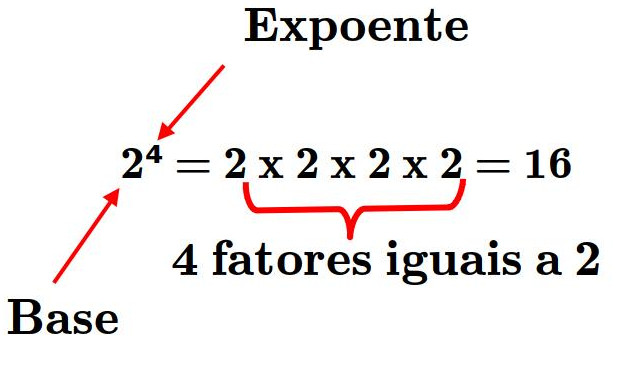
\includegraphics[scale=0.4]{potenciacao2.jpg}
 
    \label{fig:my_label}
\end{figure}
Muitos estudantes confundem a potenciação de números naturais com a multiplicação de números naturais. A multiplicação de números naturais representa uma adição de parcelas iguais. Já a potenciação representa uma \textbf{multiplicação de fatores iguais}. Observe. 
\begin{equation}
  2 \times 4 = 8  
\end{equation}
\begin{equation}
    2^4 = 16
\end{equation}
\subsection{Exemplos}
\begin{enumerate}
    \item $5^3 = 5 \cdot 5 \cdot = 125 5$
    \item $7^2 = 7 \cdot 7 = 49 $
    \item $3^4 =3 \cdot 3 \cdot 3 \cdot 3 = 81$
    \item $2^5 = 2 \cdot 2 \cdot 2 \cdot 2 \cdot 2 = 32$
\end{enumerate}
\subsection{Observações}
\begin{itemize}
    \item Quando o expoente é 2, costumamos chamar a potência de quadrado. Por exemplo, $3^2$ é lido como \textbf{três elevado ao quadrado}.
   
    \item Quando o expoente é 3, a potência recebe o nome de cubo do valor da base. Por exemplo, $5^3$ é lido como \textbf{cinco ao cubo}. 
    \item Todo número natural elevado a 1 é igual a ele mesmo. 
     $$2^1 = 2$$.
    \item Todo número natural, diferente de zero, elevado a zero é igual a 1. 
    $$0^2 = 0$$
    \item O número zero elevado a qualquer outro número natural diferente de zero é igual a zero. 
    $$2^0 = 1$$
    $$1000^0 = 1$$
    \item Zero elevado a zero é uma \textbf{indeterminação matemática}. 
\end{itemize}
\section{Decomposição de números naturais}
Uma importante aplicação da potenciação de números naturais está na decomposição desses números a partir das potências de base 10. Em um número natural, cada algarismo assume um \textbf{valor posicional}, dependendo da posição onde ele se encontra no número. Os exemplos a seguir mostram como decompor números naturais em potências de base 10. 
\subsection{Exemplos}
\begin{enumerate}
    \item $125 = 100 + 20 + 5  = 1 \cdot 10^2 + 2\cdot 10^1 + 5 \cdot 10^0$
    \item $2348 = 2000 + 300 + 40 + 8  = 2 \cdot 10^3 + 3 \cdot 10^2 + 4 \cdot 10^1 8 \cdot 10^0$ 
    \item $543 =500 + 40 + 3 = 5 \cdot 10^2 + 4 \cdot 10^1 + 3 \cdot 10^0$ 
\end{enumerate}
\end{document}